\chapter{Results}
\label{chap:results}

The results of a query : \textit{"Show me some red blazers. They are for men"} are as follows:

\begin{figure}[H]
\centering
    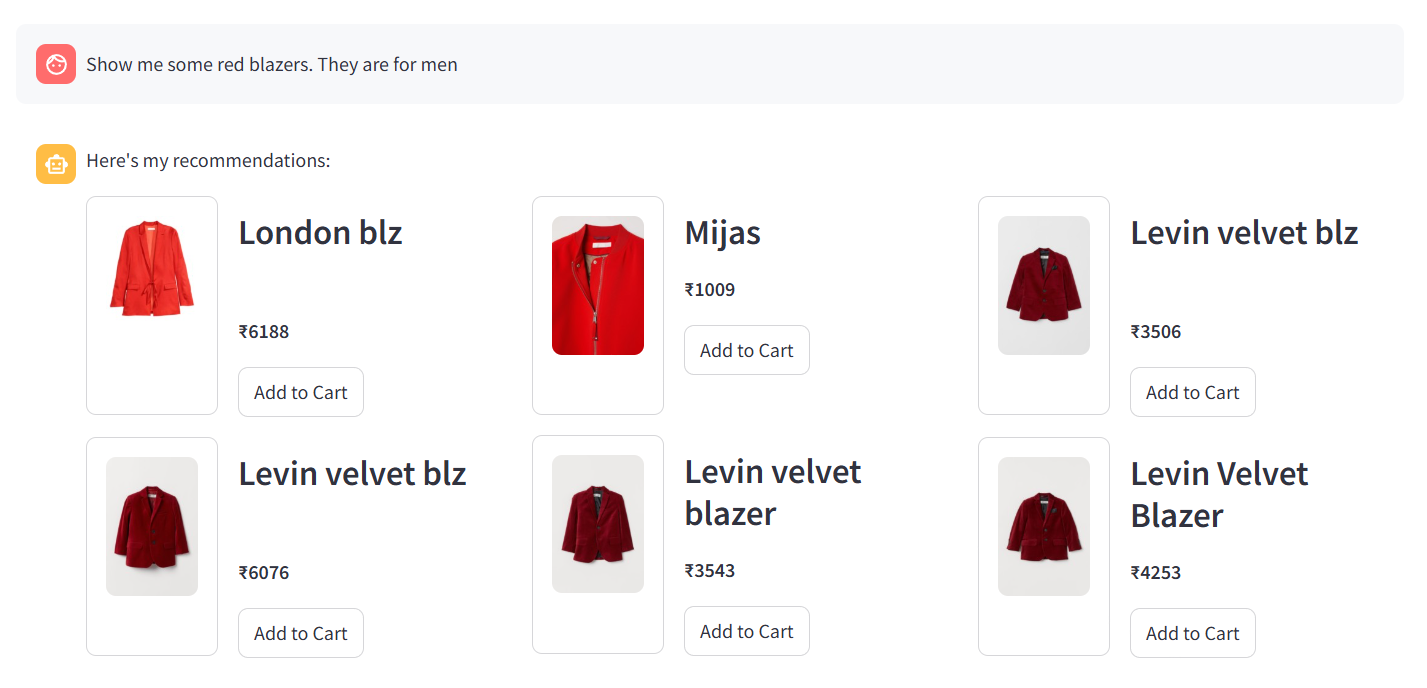
\includegraphics[width=0.8\textwidth]{images/text_srch.png}
\end{figure}

Some other examples of text based queries are shown below:

\begin{figure}[H]
\centering
    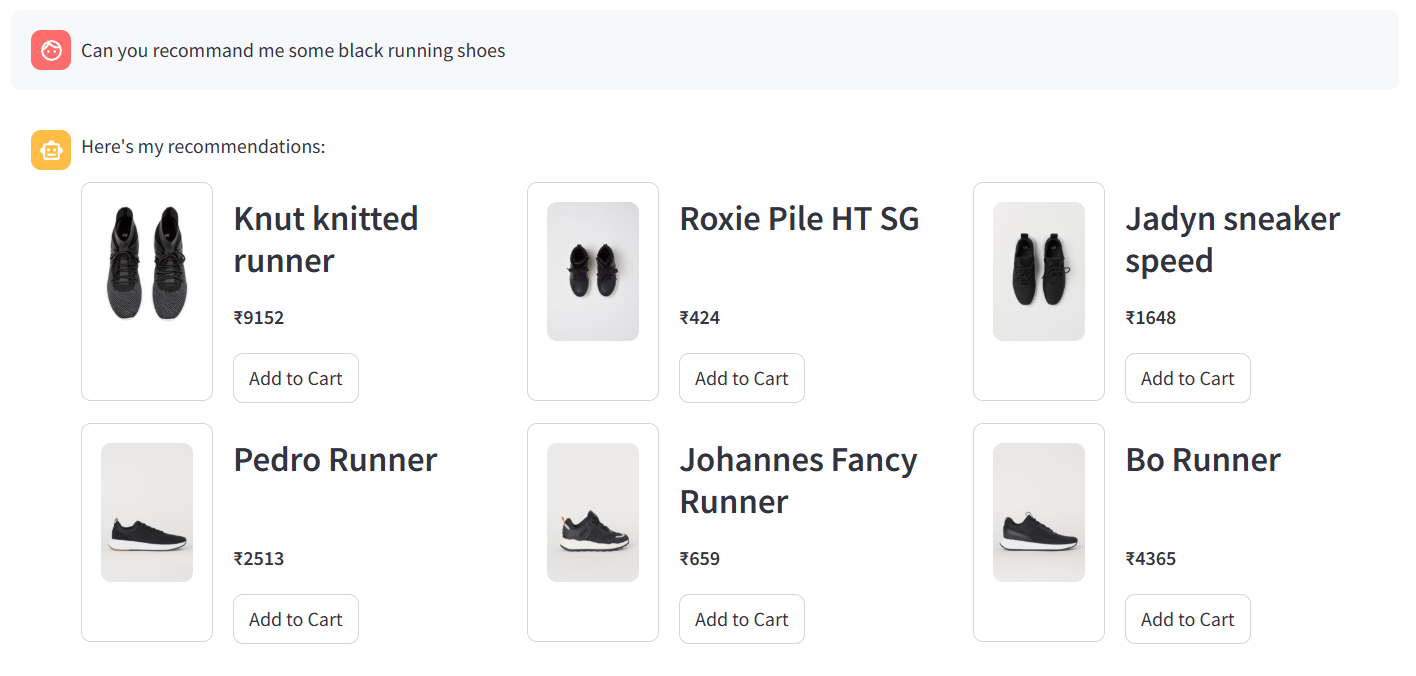
\includegraphics[width=0.8\textwidth]{images/text_srch2.png}
\end{figure}

\begin{figure}[H]
\centering
    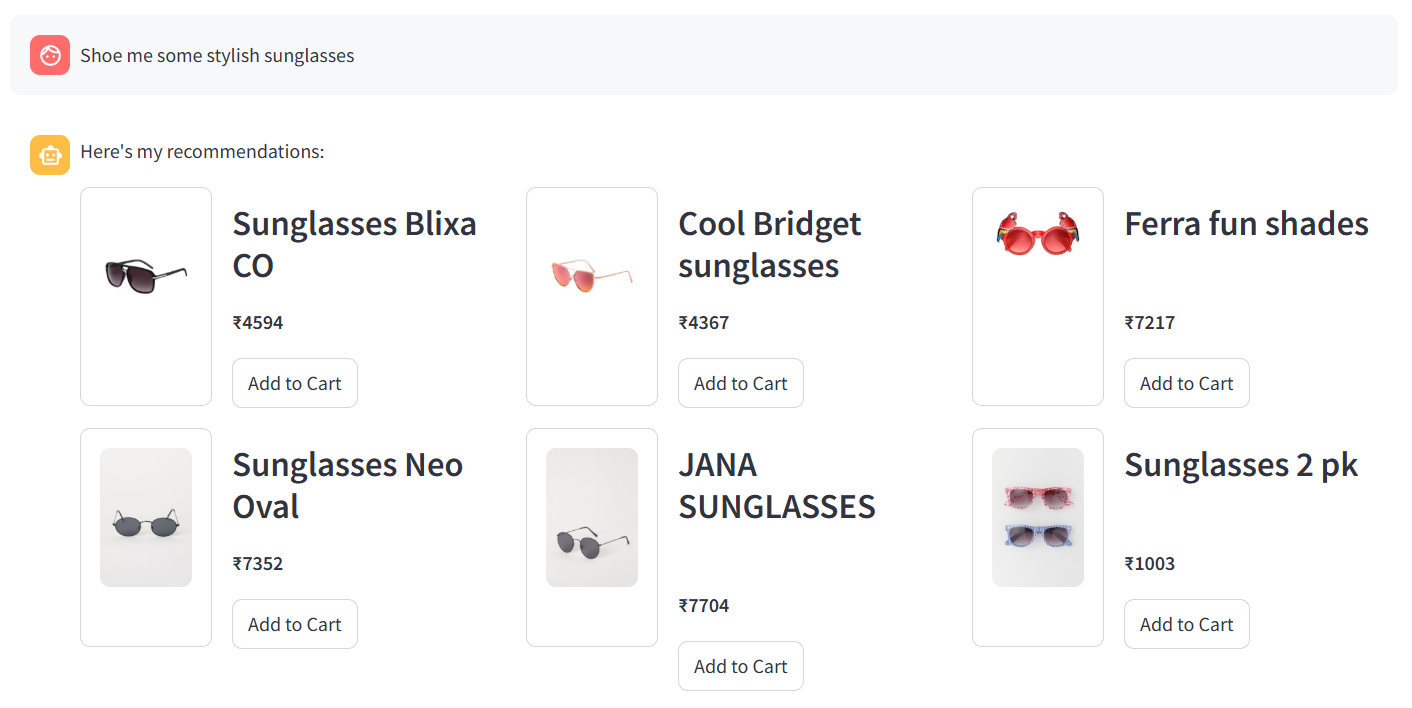
\includegraphics[width=0.8\textwidth]{images/text_srch3.png}
\end{figure}

Similarly, for a image based query, we detect the bounding boxes around the clothes in the image and then use the detected bounding boxes to crop the image. The cropped images are then used to query the fashion-clip model. The results are as follows:


\begin{figure}[H]
  \centering
  \begin{subfigure}[b]{0.3\textwidth}
      
\includegraphics[width=\textwidth]{images/og_image.png}
      \caption{Original Image}
  \end{subfigure}
  \begin{subfigure}[b]{0.3\textwidth}
      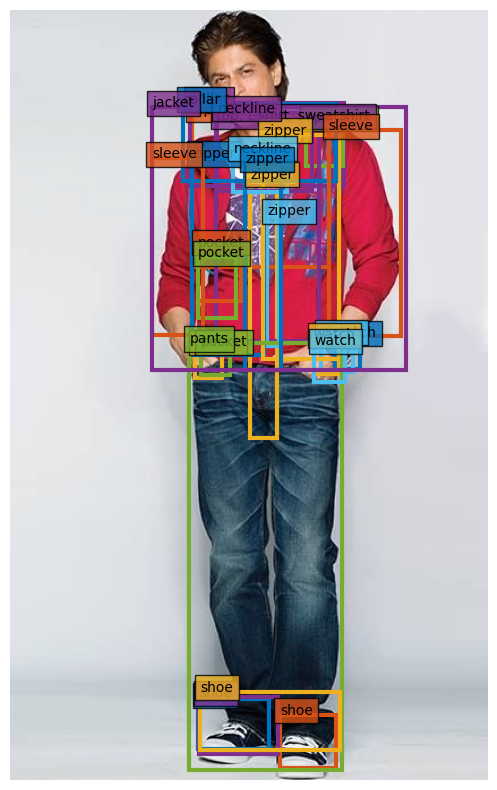
\includegraphics[width=\textwidth]{images/detected_imgae.png}
      \caption{Clothes Detected}
  \end{subfigure}
  \begin{subfigure}[b]{0.2\textwidth}
      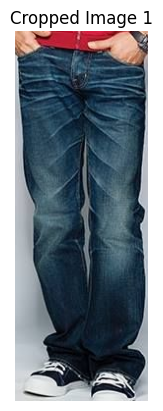
\includegraphics[width=\textwidth]{images/cropped_image.png}
      \caption{Cropped only Shirt}
  \end{subfigure}
\end{figure}

\begin{figure}[H]
  \centering
  \begin{subfigure}[b]{0.19\textwidth}
      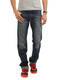
\includegraphics[width=\textwidth]{images/output1.jpeg}
      \caption{Match 1}
  \end{subfigure}
  \begin{subfigure}[b]{0.19\textwidth}
      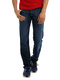
\includegraphics[width=\textwidth]{images/output2.jpeg}
      \caption{Match 1}
  \end{subfigure}
  \begin{subfigure}[b]{0.19\textwidth}
      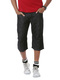
\includegraphics[width=\textwidth]{images/output3.jpeg}
      \caption{Match 1}
  \end{subfigure}
  \begin{subfigure}[b]{0.19\textwidth}
      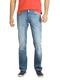
\includegraphics[width=\textwidth]{images/output4.jpeg}
      \caption{Match 1}
  \end{subfigure}
  \begin{subfigure}[b]{0.19\textwidth}
      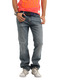
\includegraphics[width=\textwidth]{images/output5.jpeg}
      \caption{Match 1}
  \end{subfigure}
  \caption{Top 5 similar items for Cropped Image.}
  \label{fig:similar_items_1}
\end{figure}

Another example is shown below.

\begin{figure}[H]
  \centering
  \begin{subfigure}[b]{0.3\textwidth}
      
\includegraphics[width=\textwidth]{images/2og_image.png}
      \caption{Original Image}
  \end{subfigure}
  \begin{subfigure}[b]{0.3\textwidth}
      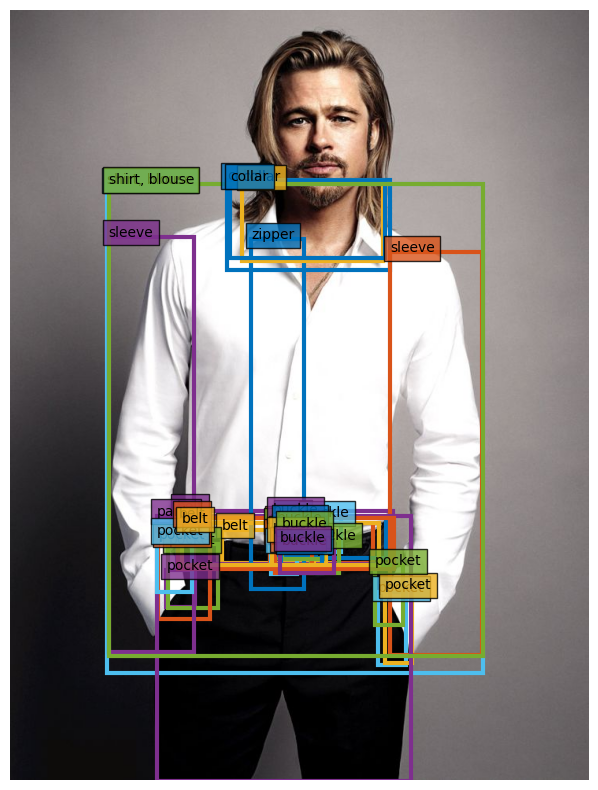
\includegraphics[width=\textwidth]{images/2detected_image.png}
      \caption{Clothes Detected}
  \end{subfigure}
  \begin{subfigure}[b]{0.2\textwidth}
      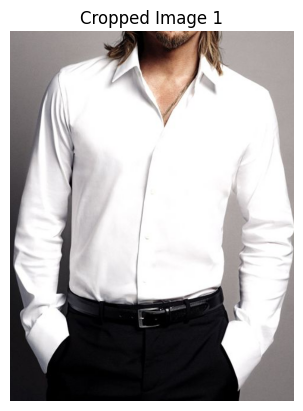
\includegraphics[width=\textwidth]{images/2cropped_image.png}
      \caption{Cropped only Pants}
  \end{subfigure}
\end{figure}

\begin{figure}[H]
  \centering
  \begin{subfigure}[b]{0.19\textwidth}
      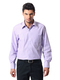
\includegraphics[width=\textwidth]{images/2output1.jpeg}
      \caption{Match 1}
  \end{subfigure}
  \begin{subfigure}[b]{0.19\textwidth}
      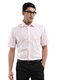
\includegraphics[width=\textwidth]{images/2output2.jpeg}
      \caption{Match 1}
  \end{subfigure}
  \begin{subfigure}[b]{0.19\textwidth}
      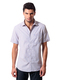
\includegraphics[width=\textwidth]{images/2output3.jpeg}
      \caption{Match 1}
  \end{subfigure}
  \begin{subfigure}[b]{0.19\textwidth}
      
\includegraphics[width=\textwidth]{images/2output4.jpeg}
      \caption{Match 1}
  \end{subfigure}
  \begin{subfigure}[b]{0.19\textwidth}
      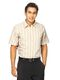
\includegraphics[width=\textwidth]{images/2output5.jpeg}
      \caption{Match 1}
  \end{subfigure}
  \caption{Top 5 similar items for Cropped Image.}
  \label{fig:similar_items_1}
\end{figure}
